\begin{frame}
  \frametitle{Qu'est-ce que l'intelligence artificielle ?}
  \pause
  \begin{itemize}
  \item Dartmouth Conference, 1956
    \begin{itemize}
    \item[] {\ptnormal{\textit{The science and engineering of making computers
            behave in ways that, until recently, we thought required human
            intelligence.}}} 
    \end{itemize}
  \item Reproduire \blue{artificiellement} les comportements du vivant
    \blue{perçus comme intelligents} \pause
  \item \blue{Effet IA: } "Intelligent est tout ce qui n'est pas encore fait par un ordinateur."\pause

  \centerline{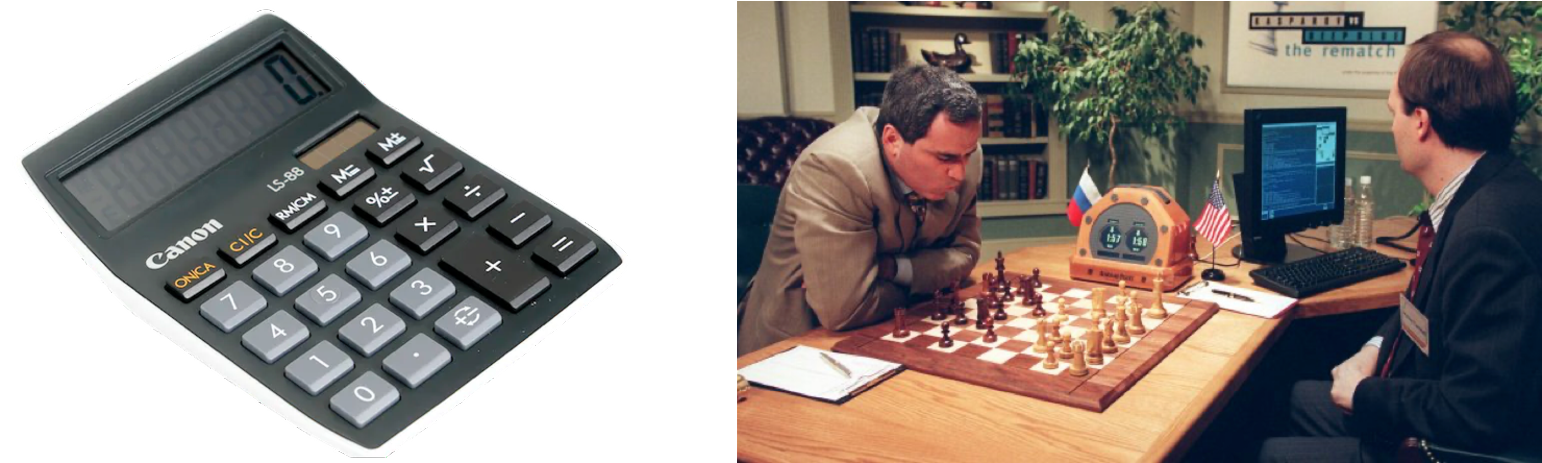
\includegraphics[width=0.75\textwidth]{intelligence}}

  % \item \black{Motivations :}
  % \begin{itemize}
  % \item \blue{Comprendre} l'intelligence naturelle ; 
  % \item Créer des \blue{outils} qui nous aident.
  % \end{itemize}
  \end{itemize}
\end{frame}

\begin{frame}
  \frametitle{Intelligence Artificielle (IA) - Motivations}
  %\centerline{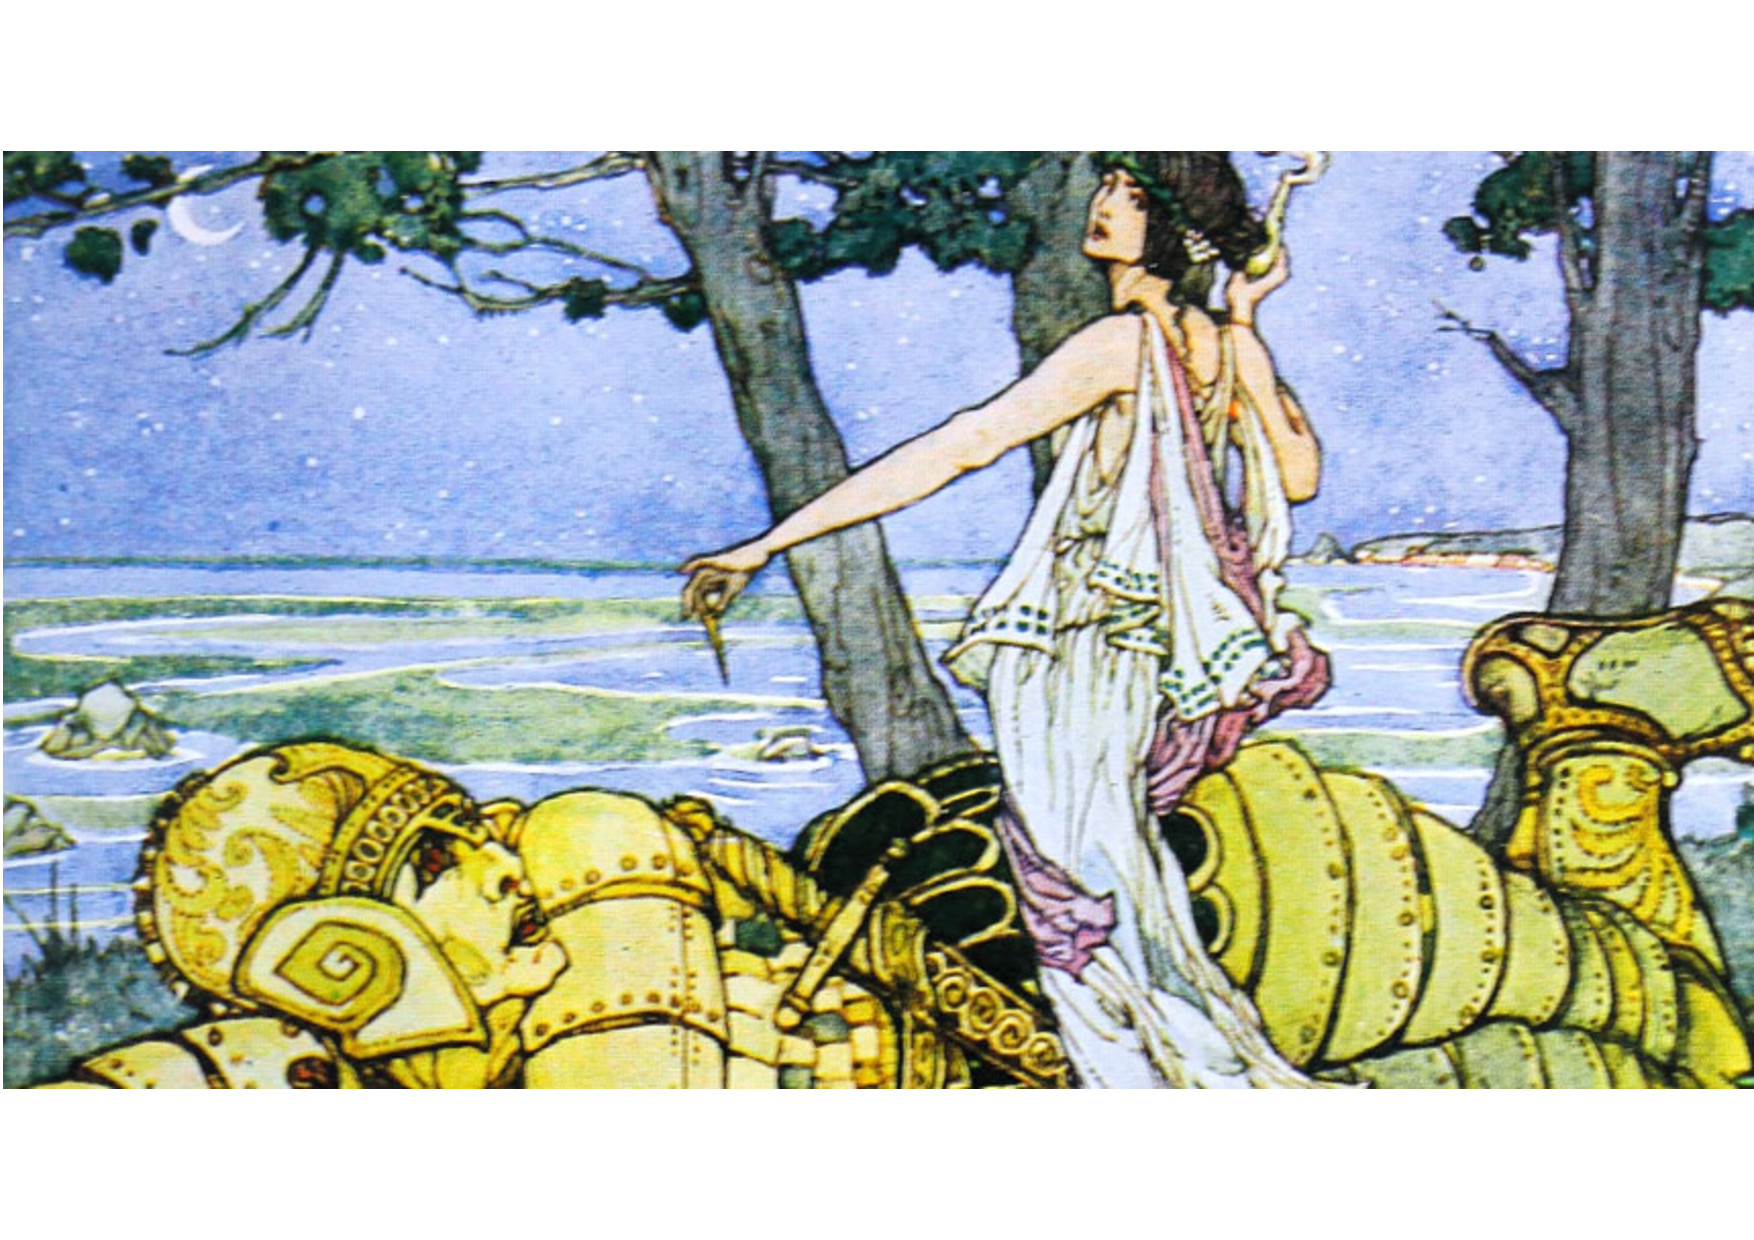
\includegraphics[width=0.6\textwidth]{mythology}}
   \begin{figure}
     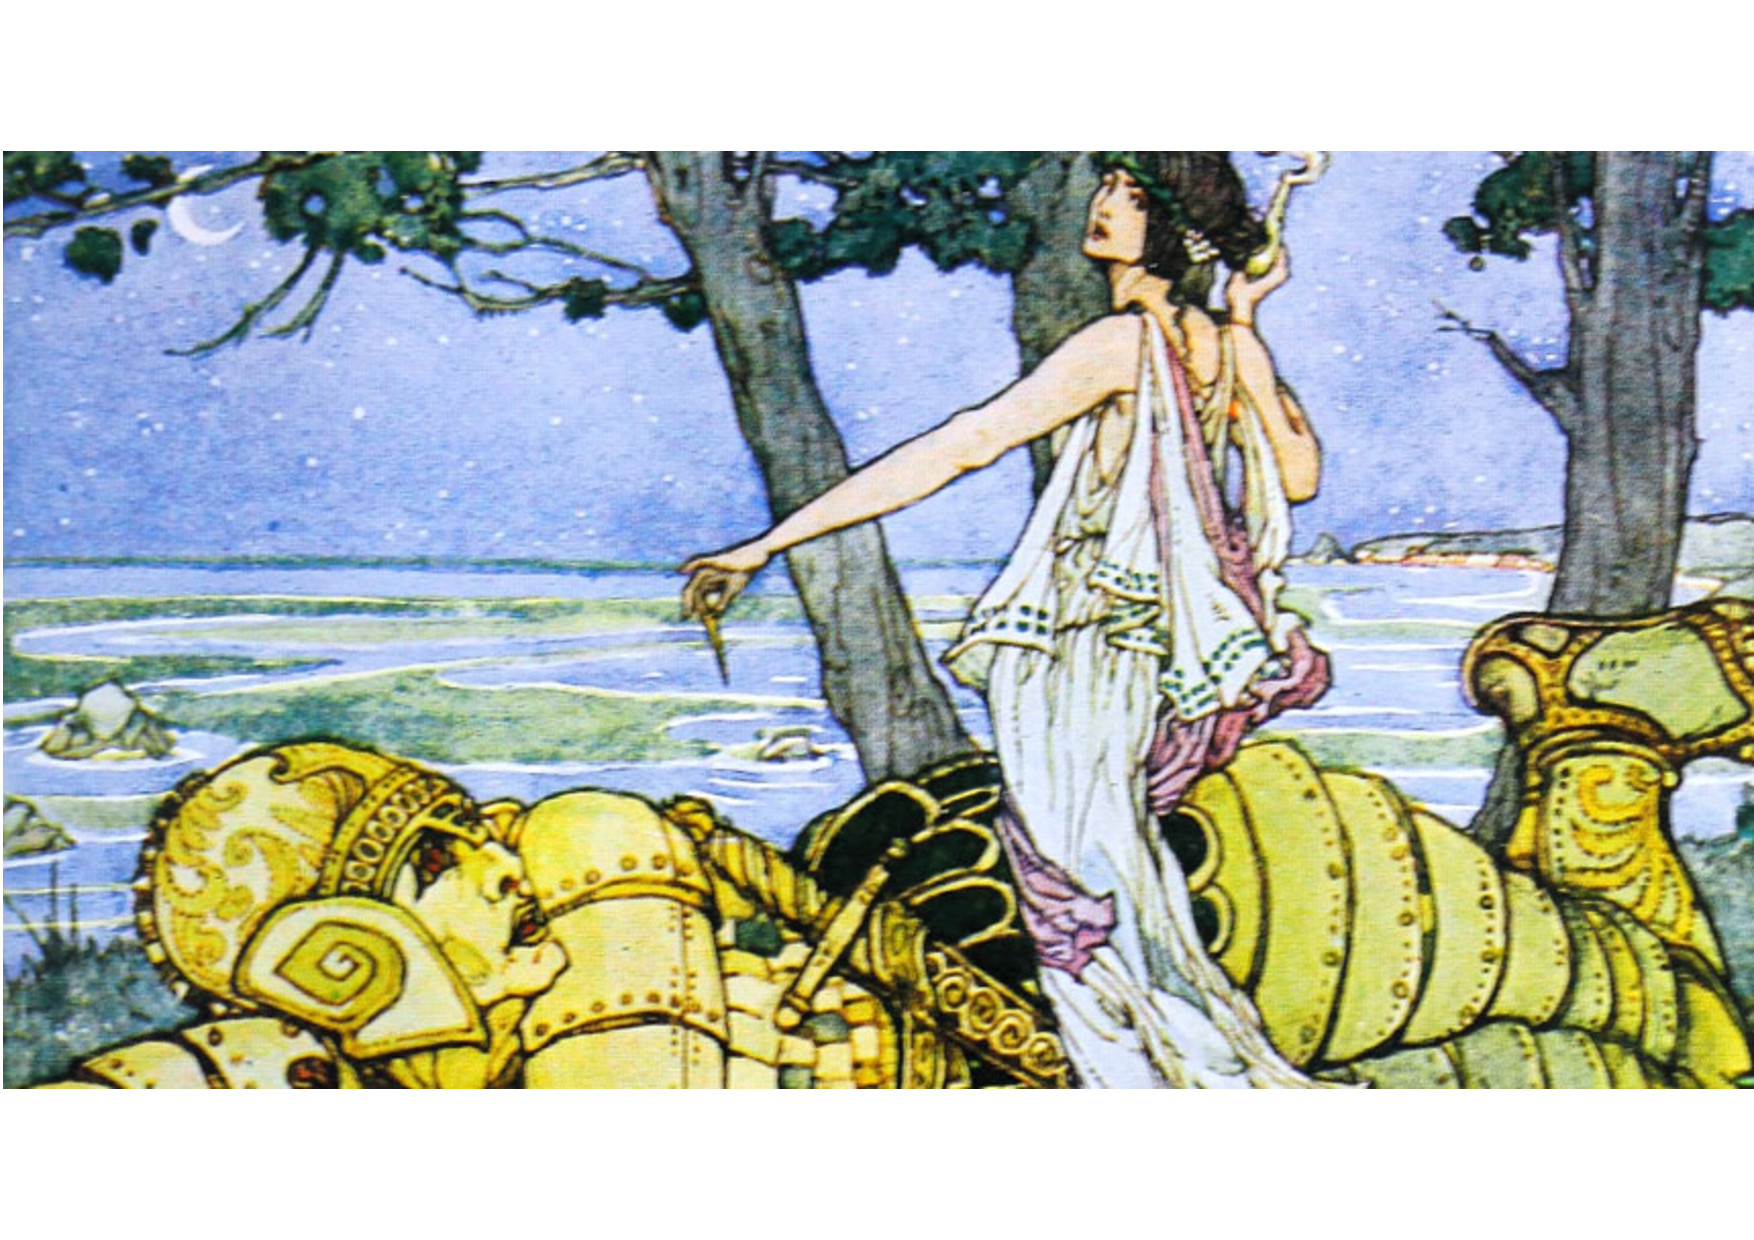
\includegraphics[width=0.5\textwidth]{mythology}
     \caption{Talos: un automate en bronze, gardien de Crète}
   \end{figure}

  \begin{itemize}

  \item Fascination scientifique
  \item Comprendre l'intelligence naturelle
  \item Outils de support dans nos tâches quotidiennes
  \begin{itemize}
    \item Automatisation
    \item Faire ce qui est infaisable pour un humain
  \end{itemize}
  % \item \black{Motivations :}
  % \begin{itemize}
  % \item \blue{Comprendre} l'intelligence naturelle ; 
  % \item Créer des \blue{outils} qui nous aident.
  % \end{itemize}
  \end{itemize}
\end{frame}


\begin{frame}
  \frametitle{Quelques sous-domaines de l'IA}
  \begin{itemize}
  \item \blue{Robotique}
    \begin{itemize}
    \item mécanique, électronique, contrôle
    \end{itemize}
  \item \blue{Systèmes experts}
    \begin{itemize}
    \item utilisent des règles 
    \item logique des propositions, logique des prédicats
    \end{itemize}
  \item \blue{Traitement du langage naturel}
  \item \blue{Vision par ordinateur}
  \item \blue{Informatique affective} 
    \begin{itemize}
    \item reconnaître, modéliser, exprimer les émotions humaines
    \item sciences cognitives, psychologie
    \end{itemize}
  \item \tikzmark{ml}{\blue{Apprentissage automatique}}
  \end{itemize}
  \pause \tikz[overlay,remember picture]{\draw[draw=MyOrange,thick]
    ($(ml)+(-0.6,0.5)$) rectangle ($(ml)+(10,-0.3)$);}
\end{frame}

\begin{frame}
  \frametitle{Apprentissage automatique}
  \begin{itemize}
  \item \red{Apprendre :}
    \pause
    acquérir une \blue{compétence} par l'\blue{expérience}, la pratique.
  \item Pour une  machine :
    \begin{itemize}
    \item \blue{compétence} = algorithme
    \item \blue{expérience,} pratique = exemples, données
    \end{itemize}
    \pause
  \item Autres noms : apprentissage statistique ; machine learning.
  \end{itemize}
\end{frame}

\begin{frame}
  \frametitle{Algorithme d'apprentissage}
  \begin{itemize}
  \item<1-> \red{Algorithme classique :}
    \begin{center}
      \begin{tikzpicture}
        \node[text width=2em] at (0.1, 5.5) {{Entrée}};
        \draw[->, draw=MyDarkGrey, thick] (0.9, 5.5) -- (1.9, 5.5);
        \draw [draw=MyBlue, thick] (2, 6) rectangle (4.5, 5) node[midway,
        align=center]{\blue{Algorithme} \\ \blue{classique}};
        \draw[->, draw=MyDarkGrey, thick] (4.6, 5.5) -- (5.6, 5.5);
        \node[text width=5em] at (6.8, 5.5) {{Sortie}};
        \pause
        \node[text width=2em] at (-.6, 4.3) {{Ingrédients}};
        \draw[->, draw=MyDarkGrey, thick] (0.9, 4.3) -- (1.9, 4.3);
        \draw [draw=MyBlue, thick] (2, 4.8) rectangle (4.5, 3.8) node[midway,
        align=center]{\blue{Recette}};
        \draw[->, draw=MyDarkGrey, thick] (4.6, 4.3) -- (5.6, 4.3);
        \node[text width=2em] at (6.3, 4.3) {{Gâteau}};
      \end{tikzpicture}
    \end{center}

  \item<3-> \red{Algorithme d'apprentissage :}
    \begin{center}
      \begin{tikzpicture}
        \node[text width=2em] at (0.1, 5.5) {{Entrée}};
        \draw[->, draw=MyDarkGrey, thick] (0.9, 5.5) -- (1.9, 5.5);
        \draw [draw=MyOrange, thick] (2, 6) rectangle (4.5, 5) node[midway,
        align=center]{\red{Algorithme} \\ \red{d'apprentissage}};
        \draw[->, draw=MyDarkGrey, thick] (4.6, 5.5) -- (5.6, 5.5);
        \node[text width=4em] at (6.8, 5.5) {\blue{Algorithme classique = modèle}};
        \pause
        \node[text width=5em, align=center] at (0, 4.3) {{Ingrédients et gâteaux}};
        \draw[->, draw=MyDarkGrey, thick] (0.9, 4.3) -- (1.9, 4.3);
        \draw [draw=MyOrange, thick] (2, 4.8) rectangle (4.5, 3.8) node[midway,
        align=center]{\red{Algorithme} \\ \red{d'apprentissage}};
        \draw[->, draw=MyDarkGrey, thick] (4.6, 4.3) -- (5.6, 4.3);
        \node[text width=2em] at (6.3, 4.3) {\blue{Recette}};
      \end{tikzpicture}
    \end{center}
  \end{itemize}  
\end{frame}

\begin{frame}
  \frametitle{Deep learning, ML et IA}
  \begin{itemize}
  \item La plupart des succès récents de l'« intelligence artificielle » sont
    en fait des progrès en \red{apprentissage automatique.}
  \item[] Il s'agit d'utiliser (beaucoup) d'exemples d'une tâche pour apprendre à faire cette
    tâche
  \item La plupart de ces progrès sont des progrès en \red{apprentissage
      profond} (deep learning) : un des domaines de l'apprentissage automatique
    qui utilise des \blue{réseaux de neurones à plusieurs couches.}
  \end{itemize}
\end{frame}

\begin{frame}
  \frametitle{Deep learning}
  \begin{itemize}
  \item \black{Exemples}
    \begin{itemize}
      \setlength{\itemsep}{5pt}
    \item \blue{Traitement automatique d'images :} reconnaître si une photo
      contient un chat / est celle d'une personne spécifique / est un
      échantillon histopathologique d'une tumeur
    \item \blue{Traitement automatique du langage :} traduction automatique,
      chatbots
    \item \blue{Génération automatique} de texte, d'images, de son, de vidéos
      réalistes (en particulier deepfakes)
    \end{itemize}
  \item \black{Ingrédients du succès :}
    \begin{itemize}
      \setlength{\itemsep}{5pt}
    \item Énormes \blue{quantités de données}
    \item \blue{Puissance de calcul}
    \item Compréhension des données et problèmes \\$\Rightarrow$ modélisation (=
      \blue{formulation} du problème) et architecture appropriées.
    \end{itemize}
  \end{itemize}
\end{frame}

\begin{frame}
  \frametitle{Autres exemples d'application du ML}
  \begin{itemize}
  \item Détection de fraude 
  \item Segmentation de marché
  \item Contrôle qualité
  \item Maintenance prédictive 
  \item Systèmes de recommendation 
  \item Trading algorithmique
  \item Assistance au diagnostic
  \item Médecine prédictive 
  \item Et beaucoup, beaucoup d'autres.
  \end{itemize}
\end{frame}

\begin{frame}
  \frametitle{Défis actuels du ML}
  \begin{itemize}
  \item Apprendre à partir de \blue{peu d'exemples}
    \begin{itemize}
    \item[] Un enfant ou un animal n'a pas besoins de milliers/millions
      d'exemples pour apprendre
    \end{itemize}
  \item Résoudre des problèmes \blue{que l'humain ne sait pas résoudre}
    \begin{itemize}
    \item[] Utilisation dans la recherche scientifique (biologie, santé,
      chimie, science des matériaux, astrophysique, etc.)
    \end{itemize}
  \item \blue{Confiance}
    \begin{itemize}
    \item[] validation formelle, explicabilité, robustesse aux attaques
  \end{itemize}
  \item \blue{Questions éthiques}
    \begin{itemize}
    \item[] biais algorithmiques ; coûts environementaux ; équité et moralité
    \end{itemize}
  \end{itemize}
\end{frame}

\begin{frame}
  \begin{center}
    \large{1. Types de problèmes d'apprentissage automatique}
  \end{center}
\end{frame}

\begin{frame}
  \frametitle{1.1 Apprentissage supervisé}
  \begin{center}
    \begin{tikzpicture}
      \tikzstyle{every node}=[font=\small]
      \node[text width=5em] at (0.1, 5.5) {Observations étiquetées};
      \draw[->, draw=MyDarkGrey, thick] (0.9, 5.5) -- (1.9, 5.5);
      \draw [draw=MyDarkGrey, thick] (2, 6) rectangle (4.5, 5)
      node[midway, text width=5em, align=center]{Algorithme d'apprentissage};
      \draw[->, draw=MyDarkGrey, thick] (4.6, 5.5) -- (5.6, 5.5);
      \node[text width=5em] at (7, 5.5) {Modèle prédictif};
    \end{tikzpicture}
  \end{center}

  \begin{itemize}
  \item \black{But :} \red{apprendre} un modèle \blue{prédictif}
  \pause
  \item \black{Formalisation :}
    \begin{itemize}
    \item[] \blue{Données :} 
    \item $n$ observations $\{\xvec_1, \xvec_2, \dots, \xvec_n\}$ ; $\xvec_i \in \xcal$ \only<2->{$= \RR^p$}
    \item $n$ étiquettes $\{y_1, y_2, \dots, y_n\}$ ; $y_i \in \ycal$ 
      \begin{itemize}
      \item<3-> \red{Régression} : $\ycal = \RR$ 
      \item<4-> \red{Classification} : $\ycal = \{0, 1, \dots, C-1\}$ 
      \item<5-> \red{Classification binaire} : $\ycal = \{0, 1\}$ 
      \end{itemize}
    \item[] \blue{Sortie :}
    \item \blue{modèle} $f: \xcal \rightarrow \ycal$ tel que $f(\xvec_i) \approx y_i$.  
    \end{itemize}
  \item<6-> \red{Inférence} :  étant donné $\xvec \in \xcal$, prédire $\hat{y} = f(\xvec)$. 
  \end{itemize}
\end{frame}

\begin{frame}
  \frametitle{Exemples}
  \begin{itemize}
  \item Exemples de \blue{problèmes de régression :}  $\ycal = \RR$ 
    \begin{itemize}
    \item \blue{Prédiction de clics :} combien de personnes vont cliquer sur ce lien ?
    \item Prédiction de la \blue{solubilité d'une molécule} dans l'éthanol en mg/mL
    \end{itemize}
  \pause
  \item Exemples de \blue{problèmes de classification binaire :}  $\ycal = \{0, 1\}$
    \begin{itemize}
    \item \blue{Filtrage de spam :} cet email est-il un spam ?
    \item \blue{Reconnaissance faciale :} est-ce JM Blanquer sur cette photo ?
    \end{itemize}
  \pause
  \item Exemples de \blue{problèmes de classification multiclasse :}  
    \begin{itemize}
    \item \blue{OCR}, reconnaissance de chiffres manuscrits : $\ycal = \{0, 1, 2, \dots, 9\}$
    \item Reconnaissance de \blue{plantes} ou de \blue{chants d'oiseaux}
    \end{itemize} 
  \end{itemize}
\end{frame}

\begin{frame}
  \frametitle{1.2 Apprentissage non supervisé}
  \begin{center}
      \begin{tikzpicture}
       \tikzstyle{every node}=[font=\small]
        \node[text width=5em] at (0.1, 5.5) {Observations non étiquetées};
        \draw[->, draw=MyDarkGrey, thick] (0.9, 5.5) -- (1.9, 5.5);
        \draw [draw=MyDarkGrey, thick] (2, 6) rectangle (4.5, 5)
        node[midway, text width=5em, align=center]{Algorithme d'apprentissage};
        \draw[->, draw=MyDarkGrey, thick] (4.6, 5.5) -- (5.6, 5.5);
        \node[text width=5em] at (7, 5.5) {Représentation des observations};
      \end{tikzpicture}
  \end{center}
  \begin{itemize}
  \item \black{But :} \red{explorer} les données ; apprendre une nouvelle représentation
  \pause
  \item \black{Formalisation :}
    \begin{itemize}
    \item[] \blue{Données :} 
    \item[] $n$ observations $\{\xvec_1, \xvec_2, \dots, \xvec_n\}$ ; $\xvec_i \in \xcal = \RR^p$
      \vspace{.5em}
    \item[] \blue{Sortie :}
    \pause
      \item \red{Réduction de dimension :} $f : \RR^p \rightarrow \RR^d$ avec
        $d \ll p$ et de telle sorte à ce que $f(\xvec)$ soit une
        \blue{représentation informative} de $\xvec$
      \pause
      \item \red{Clustering :} partition de $\{1, 2, \dots, n\}$ en ensembles
        d'éléments semblables, appelés \red{clusters}
      \pause
      \item \red{Estimation de densité :} la loi de probabilité de $X$ dont
        $\{\xvec_1, \xvec_2, \dots, \xvec_n\}$ est supposé être un échantillon.
    \end{itemize}
  \end{itemize}
\end{frame}

\begin{frame}
  \frametitle{Réduction de dimension}
  \begin{itemize}
  \item[] Apprendre $f : \RR^p \rightarrow \RR^d$ avec $d \ll p$ et de telle
    sorte à ce que $f(\xvec)$ soit une \blue{représentation informative} de
    $\xvec$
  \item \black{Utilisation :}
    \begin{itemize}
    \item Visualiser les données (en particulier $d=2$)
    \item Réduire la taille des données en mémoire
    \item Améliorer la performance d'un algorithme supervisé
    \end{itemize}
  \end{itemize}
\end{frame}

\begin{frame}
  \frametitle{Clustering}
  \begin{itemize}
  \item[] Apprendre une partition de $\{1, 2, \dots, n\}$ en ensembles
    d'éléments semblables, appelés \red{clusters}
  \item \black{Exemples d'application :}
    \begin{itemize}
    \item \blue{Segmentation de marché :} regrouper des clients qui ont des
      profils similaires
    \item \blue{Topic modeling: } regrouper les documents d'un corpus par
      thème ; les thèmes émergent de l'analyse et ne sont pas fournis. %(sans les fournir)
    \end{itemize}
  \end{itemize}
\end{frame}


  \begin{frame}
  \frametitle{1.3 Autres problèmes d'apprentissage}
  
  \begin{itemize}
  \item \red{Apprentissage semi-supervisé}
    \begin{itemize}
    \item[] Une partie seulement des données est étiquetée
    \end{itemize}
  \item \red{Apprentissage par renforcement}
    \begin{itemize}
    \item[] Définir une \blue{politique} permettant de maximiser sa \blue{récompense} 
    \end{itemize}
  \item \red{Régression structurée}
    \begin{itemize}
    \item[] Apprentissage supervisé avec $\ycal$ un espace de vecteurs, de
      séquences, de texte, de graphes etc.
    \end{itemize}
  \end{itemize}
\end{frame}

\begin{frame}
  \begin{center}
    \large{2. Premier exemple : les plus proches voisins}
  \end{center}
\end{frame}

\begin{frame}
  \frametitle{2.1 Algorithme du plus proche voisin}
  \begin{overlayarea}{\textwidth}{\textheight}
  \begin{itemize}
  \item<1-> \blue{Données :} $\dset = \{(\xvec_1, y_1), (\xvec_2, y_2), \dots, (\xvec_n, y_n)\} $ 
    \begin{itemize}
    \item $n$ observations en $p$ dimensions : $\xvec_i \in \RR^p$
    \item $n$ étiquettes : $y_i \in \ycal$
    \end{itemize}
  \item<2-> \blue{Modèle :} Associer à $\xvec \in \RR^p$ l'étiquette de l'exemple
    dans $\dset$ dont $\xvec$ est le plus proche selon la distance euclidienne
  \[ f(\xvec) = y_{\argmin_{i=1, \dots, n} \ltwonorm{\xvec - \xvec_i}} \]
    \only<3>{\centering 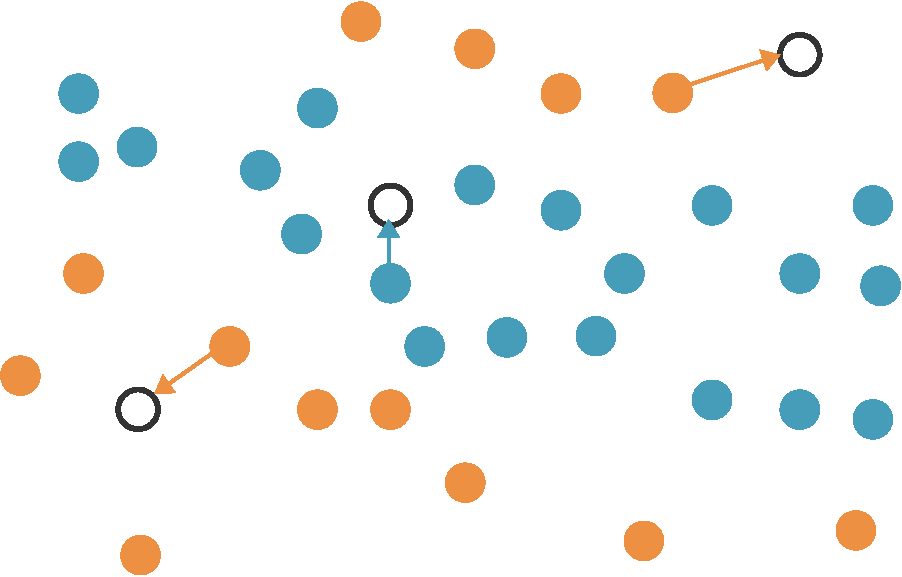
\includegraphics[width=0.45\textwidth]{figures/nearest_neighbor}}
    \item<4-> Régression, classification binaire, classification multiclasse.
    \item<5-> \red{Pas de phase d'apprentissage !}
    \end{itemize}
  \end{overlayarea}
\end{frame}

\begin{frame}
  \frametitle{2.2 kNN pour la classification}
  \begin{itemize}
  \item L'algorithme du plus proche voisin est \blue{peu robuste} au bruit
  \item Plutôt que d'utiliser \blue{le} plus proche voisin : utiliser les $k$
    observations les plus proches
  \item \red{Vote de la majorité :} on donne à $\xvec$ 
    \blue{l'étiquette majoritaire} parmi ses $k$ plus proches voisins
    \pause
      \begin{mdframed}[hidealllines=true, backgroundcolor=MyLightGrey,
                       fontcolor=MyDarkGrey, leftmargin=-5pt,
                       innerleftmargin=5pt, skipabove=5pt]
    \[ f(\xvec) = \argmax_{c \in \{0, 1, \dots, C-1\}} \sum_{i : \xvec_i \in \ncal_k(\xvec)} \delta(y_i, c) \]
      \begin{itemize}
      \item $\ncal_k(\xvec)$ est l'ensemble des $k$ plus proches voisins de $\xvec$ dans $\dset$
      \item $\delta(y_i, c) = 1$ si $y_i = c$ et $0$ sinon; $C$ est le nombre de classes.
      \end{itemize}
    \end{mdframed}
  \pause
  \item Pour la classification binaire, on utilise un nombre \blue{impair} de voisins pour ne pas avoir d'ex-aequo.
  \end{itemize}
\end{frame}

\begin{frame}
  \frametitle{2.3 kNN pour la régression}
  \begin{itemize}
  \item \red{Moyenne :} on donne à $\xvec$ 
    \blue{la moyenne des étiquettes} de ses $k$ plus proches voisins
    \[ f(\xvec) = \frac1k \sum_{i : \xvec_i \in \ncal_k(\xvec)} y_i \]
  \end{itemize}
  \pause
    \begin{itemize}
    \item \black{Remarque :} Les modèles donnés par des algorithmes de plus
      proches voisins sont des modèles \red{non-paramétriques :}
      \begin{itemize}
      \item il ne s'agit pas d'apprendre les paramètres d'une expression explicite des variables
        $x_1, \dots, x_p$
      \item par opposition aux \blue{modèles linéaires} et aux \blue{réseaux de neurones}
      \item $k$ est un \red{hyperparamètre} : l'algorithme ne permet pas de l'apprendre.
      \end{itemize}
    \end{itemize}
  % \end{mdframed}
\end{frame}

{\setbeamercolor{background canvas}{bg=MyLightGrey}
  \begin{frame}
    \frametitle{2.4 Variantes}
    \begin{itemize}
    \item \blue{Epsilon-voisins} Au lieu de considérer $k$ voisins les plus
      proches, on considère toutes les observations contenues dans une boule de
      rayon $\epsilon$ centrée sur $\xvec$.
    \item \blue{Pondérations des voisins} La contribution de chaque voisin est
      pondérée par un coefficient inversement proportionnel à sa distance à
      $\xvec$.
    \item \blue{Autres distances} L'algorithme s'applique aussi en considérant
      d'autres distances / notions de similarité :
      \begin{itemize}
      \item Distance de Minkowski
      \item Similarité cosinus
      \item Distance de Hamming entre vecteurs binaires
      \end{itemize}
    \end{itemize}
  \end{frame}}




%%% Local Variables:
%%% mode: latex
%%% TeX-master: "2022-01-azencott"
%%% End:
